\documentclass[letterpaper]{article} % DO NOT CHANGE THIS
\usepackage{aaai2027}  % DO NOT CHANGE THIS
\usepackage[hyphens]{url}  % DO NOT CHANGE THIS
\usepackage{graphicx} % DO NOT CHANGE THIS
\urlstyle{rm} % DO NOT CHANGE THIS
\def\UrlFont{\rm}  % DO NOT CHANGE THIS
\usepackage{natbib}  % DO NOT CHANGE THIS AND DO NOT ADD ANY OPTIONS TO IT
\usepackage{caption} % DO NOT CHANGE THIS AND DO NOT ADD ANY OPTIONS TO IT
\frenchspacing  % DO NOT CHANGE THIS

% Math and table support (all permitted by aaai2027.sty).
\usepackage{amsmath}
\usepackage{amssymb}
\usepackage{booktabs}
\usepackage{multirow}

% Keep the \pdfinfo as shown here. There's no need
% for you to add the /Title and /Author tags.
\pdfinfo{
/TemplateVersion (2027.1)
}

% Numbered sections and subsections (required so that the Section~\ref{...}
% cross-references in the text render with numbers). Do not raise above 2.
\setcounter{secnumdepth}{2}

% Title
\title{Band Depth Uncertainty Quantification for Chain-of-Thought Reasoning in Large Language Models}
\author{
    Anonymous Submission
}
\affiliations{
    Anonymous Institution\\
    anonymous@example.com
}

\begin{document}

\maketitle

% -----------------------------------------------------------------------
\begin{abstract}
Chain-of-Thought (CoT) prompting has become the dominant paradigm for eliciting
reasoning from large language models (LLMs), yet it has created a widening gap
in uncertainty quantification (UQ). When a model generates a step-by-step
reasoning chain, it exposes far richer information than just a final answer---
but existing black-box UQ methods discard this structure entirely, reducing
reliability estimation to counting how often sampled final answers agree.
This is insufficient: two chains that reach the same answer via structurally
divergent reasoning paths are not equally trustworthy, yet answer-level
consistency treats them identically. Approaches that ask the model to verbalize
its own confidence fare no better, yielding scores barely above chance
(AUROC\,$\approx$\,0.50--0.55 in our experiments). The core problem is that
meaningful uncertainty signals are latent in the \emph{geometry} of the
reasoning process---in where chains converge, where they diverge, and how
central each chain is relative to the ensemble---and neither answer-level
counting nor verbal introspection can access that geometry.

We propose \textbf{BD-UQ}, a family of truly black-box UQ methods that operate
directly on the structure of CoT reasoning ensembles using \emph{Band Depth}
(BD), a classical concept from functional data analysis that measures how
centrally a curve lies within a distribution of curves. We lift band depth from
ordered curves to discrete reasoning paths by building a \emph{reasoning graph}
over an ensemble of sampled CoT chains: nodes are semantic clusters of reasoning
steps and edges capture sequential or cross-chain semantic proximity. Three
variants exploit this graph at increasing levels of sophistication---\textbf{pBD}
operates on aligned paths, \textbf{vBD} on individual graph vertices, and
\textbf{gBD} on random walks that explore the full topology of the reasoning
space beyond the specific chains generated. All variants require only a small
sentence encoder and zero additional LLM calls. Extensive experiments across
mathematical reasoning and multi-hop question answering benchmarks show that
gBD consistently and substantially outperforms sampling-based and verbalized
baselines, demonstrating that the reasoning graph is a powerful and previously
untapped source of uncertainty signal.
\end{abstract}

% -----------------------------------------------------------------------
\section{Introduction}
\label{sec:intro}

\begin{figure}[t]
  \centering
  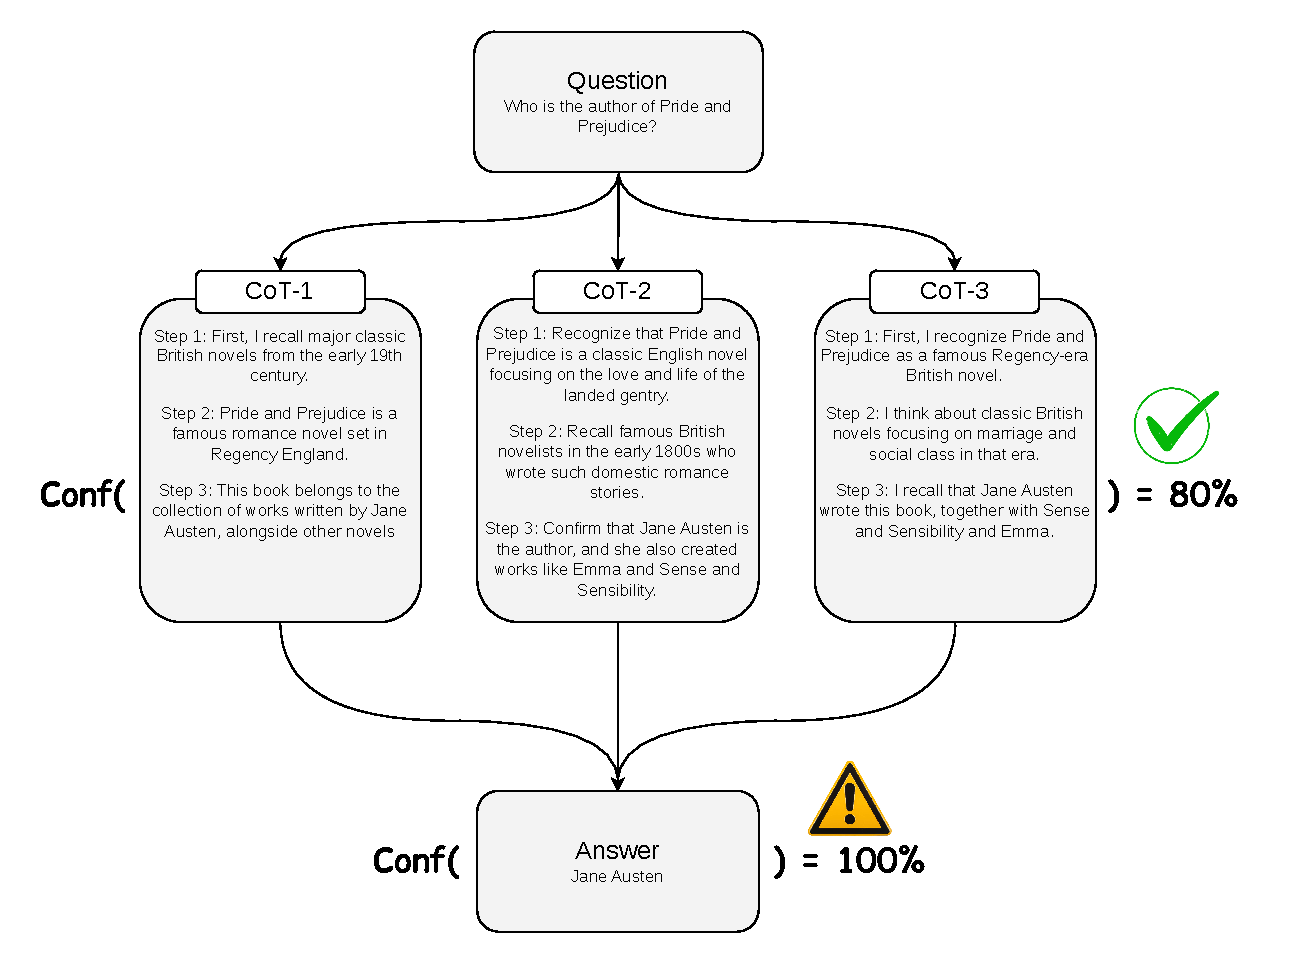
\includegraphics[width=0.95\columnwidth]{resources/intro_motivation}
  \caption{Answer-level versus reasoning-level uncertainty. A question is sampled
  into several Chain-of-Thought responses that all reach the same final answer
  (``Jane Austen''), so answer-level agreement reports full---and
  overconfident---certainty ($\mathrm{Conf(ans)}=100\%$). Yet the three chains
  reason along visibly different paths, so the reasoning itself is far less
  certain ($\mathrm{Conf(CoT)}=80\%$). Our band-depth methods score exactly this
  reasoning diversity, which answer-level agreement discards.}
  \label{fig:intro}
\end{figure}

Large language models (LLMs) have become capable general-purpose reasoners, in
large part due to Chain-of-Thought (CoT) prompting~\citep{wei2022chain}, which
elicits explicit step-by-step reasoning before a final answer and has driven
strong gains on mathematical and multi-hop reasoning tasks~\citep{wang2023selfconsistency, yao2023tree}.
As these models are deployed in increasingly consequential settings, however,
their fluent but sometimes confidently wrong outputs make it essential to know
\emph{when to trust} a given response. Uncertainty quantification (UQ) addresses
this by attaching a confidence score to each generation, ideally one that ranks
correct answers above incorrect ones. The most practically important regime is
\emph{black-box} UQ, where only the generated text is available---no token
logits, hidden states, or gradients---since this is the only access mode offered
by the strongest proprietary models and the cheapest to deploy for open ones.

Existing black-box UQ methods almost universally reduce a response to its
\emph{final answer} and measure agreement across multiple sampled answers.
Self-consistency counts how often the majority answer recurs~\citep{wang2023selfconsistency};
semantic entropy clusters answers by meaning and measures the entropy of the
cluster distribution~\citep{kuhn2023semantic, farquhar2024detecting};
and related approaches compute pairwise answer similarity or
non-contradiction~\citep{lin2023generating, manakul2023selfcheckgpt, chen2024quantifying}.
A second line of work instead asks the model to \emph{verbalize} its own
confidence, either directly or by self-probing in a fresh
context~\citep{xiong2024llms, liu2024uait}. Both families have a common
blind spot: they treat the reasoning chain---the very structure CoT was designed
to produce---as a black box. Answer-level methods discard it entirely, and
verbalized methods rely on the model's unreliable introspection over it.



This blind spot matters because the reasoning chain carries information that the
final answer cannot. As illustrated in Figure~\ref{fig:intro}, two responses may
converge on the same answer through entirely different reasoning paths---one
sound, one a lucky coincidence of errors---yet answer-level consistency assigns
them identical confidence.
Conversely, an ensemble whose chains disagree sharply at intermediate steps
signals genuine model uncertainty even when the final answers happen to match.
Recent work has begun to incorporate reasoning into UQ: CoT-UQ extracts
keywords and importance scores from each step to reweight token
probabilities~\citep{zhang2025cotuq}, and graph-based metrics summarize
relationships among extracted claims~\citep{jiang2024graphuncertainty}. Yet
CoT-UQ still requires token logits (and is therefore not fully black-box) and
operates on a single response rather than an ensemble, while claim-graph methods
target long-form factuality rather than the geometry of reasoning itself. The
question of how to extract uncertainty from the \emph{structure} of an ensemble
of reasoning chains, using text alone, remains open.

We argue that the right signal lives in the \emph{geometry} of the reasoning
ensemble: where chains converge, where they diverge, and how central each chain
is relative to the others. To capture this, we turn to \emph{band depth}, a
concept from functional data analysis that ranks a set of curves from most
central (the functional median) to most outlying~\citep{lopezpintado2009banddepth},
and which has been extended to ensembles of contours and of paths on a
graph~\citep{santer2023contourbanddepth, raj2017pathboxplots}. Building on this
lineage, we embed every reasoning step of every sampled chain with a sentence
encoder~\citep{reimers2019sentencebert} and construct a \emph{reasoning graph}
whose nodes are semantic clusters of steps and whose edges encode sequential and
cross-chain proximity. On this graph we define a family of depth-based
confidence scores---\textbf{pBD}, \textbf{vBD}, and \textbf{gBD}---that measure
how central each chain is within the ensemble. A chain that lies deep inside the
ensemble's reasoning band is trustworthy; an outlying chain is not. Crucially,
all variants are fully black-box and model-free: they require only the sampled
text and a lightweight encoder, with no additional LLM calls.

Our contributions are as follows:
\begin{itemize}
  \item \textbf{Conceptually}, we identify the structure of CoT reasoning
        ensembles as an untapped source of black-box uncertainty, and show that
        the geometric notion of band depth provides a principled way to exploit
        it---going beyond both answer-level consistency and verbalized
        self-probing.
  \item \textbf{Technically}, we introduce a reasoning-graph construction over
        sampled CoT chains and three band-depth confidence estimators on it:
        \textbf{pBD} (path-level, order-sensitive), \textbf{vBD} (vertex-level,
        order-invariant), and \textbf{gBD} (path-level via random walks,
        order-invariant), each requiring no token logits and no extra LLM
        inference.
  \item \textbf{Empirically}, we evaluate on five benchmarks across mathematical
        reasoning~\citep{cobbe2021gsm8k, patel2021svamp, miao2020asdiv} and
        multi-hop question answering~\citep{yang2018hotpotqa, ho2020wikimultihop}
        with two Llama models~\citep{touvron2023llama2, grattafiori2024llama3},
        showing that gBD consistently and substantially outperforms
        sampling-based and verbalized baselines.
\end{itemize}

The remainder of this paper is organized as follows. Section~\ref{sec:prelim}
formalizes the black-box UQ problem and the CoT generation format.
Section~\ref{sec:method} constructs the reasoning graph and defines the pBD,
vBD, and gBD estimators. Section~\ref{sec:related} situates our work within the
UQ and CoT literature. Section~\ref{sec:exp} reports experimental setup,
results, and ablations, and we conclude thereafter.

% -----------------------------------------------------------------------
\section{Preliminaries}
\label{sec:prelim}

\paragraph{Problem setup.}
Let $\mathcal{M}$ denote a black-box LLM: given a prompt $x$, it returns a
response $y \sim \mathcal{M}(\cdot \mid x)$, and we assume access only to its
generated text. For a dataset
$\{x_i\}_{i=1}^{N}$ with reference answers $\{y_i^\star\}_{i=1}^{N}$, an oracle
correctness function $h(y_i; y_i^\star) \in \{0, 1\}$ indicates whether response
$y_i$ is correct; this label is used only for offline evaluation and is
unavailable at inference time. The goal of uncertainty quantification (UQ) is to design a confidence scorer
\begin{equation}
  \hat{s}: y_i \mapsto \hat{s}(y_i)\in[0,1],
\end{equation}
that assigns higher scores to correct responses than to incorrect ones.
Because $\hat{s}$ depends only on model outputs and never on $y_i^\star$, it
serves as a practical proxy for the inaccessible oracle.

\paragraph{Chain-of-Thought generation.}
Under Chain-of-Thought (CoT) prompting~\citep{wei2022chain}, a response is not a
bare answer but a structured reasoning trace. We write a CoT response as an
ordered sequence of reasoning steps followed by a final answer,
\begin{equation}
  y_i = (s_1, s_2, \ldots, s_k, a),
\end{equation}
where each $s_j$ is a natural-language reasoning step and $a$ is the extracted
final answer. Throughout, we refer to the step sequence
$P = (s_1, \ldots, s_k)$ as a \emph{reasoning chain} (or path) and to $a$ as its
answer.

\paragraph{Ensemble of reasoning chains.}
Rather than scoring a single response, our methods operate on an \emph{ensemble}
of CoT responses sampled for the same prompt. For each $x_i$, we draw $M$
responses under stochastic decoding,
\begin{equation}
  \{ y_i^{(1)}, \ldots, y_i^{(M)} \} \sim \mathcal{M}(\cdot \mid x_i),
  \qquad
  y_i^{(m)} = (P_i^{(m)}, a_i^{(m)}),
\end{equation}
yielding $M$ reasoning chains $\{P_i^{(m)}\}_{m=1}^{M}$ and their answers
$\{a_i^{(m)}\}_{m=1}^{M}$. Answer-level baselines summarize only the multiset of
answers $\{a_i^{(m)}\}$; in contrast, our methods (Section~\ref{sec:method})
exploit the full set of chains $\{P_i^{(m)}\}$. We embed each reasoning step with
a frozen sentence encoder~\citep{reimers2019sentencebert}, mapping a step $s$ to
a vector $e(s) \in \mathbb{R}^d$, which provides the geometric substrate on
which band depth is computed.

\paragraph{Evaluation metric.}
Following standard practice in LLM UQ~\citep{kuhn2023semantic, xiong2024llms}, we
evaluate confidence scorers by the Area Under the Receiver Operating
Characteristic curve (AUROC) between the predicted scores $\{\hat{s}(y_i)\}$ and
the binary correctness labels $\{h(y_i; y_i^\star)\}$. AUROC measures the
probability that a randomly chosen correct response receives a higher confidence
than a randomly chosen incorrect one; a score of $1.0$ is perfect ranking and
$0.5$ corresponds to random guessing, with no dependence on a particular
threshold $\tau$.

% -----------------------------------------------------------------------
\section{Methodology}
\label{sec:method}

\begin{figure*}[t]
  \centering
  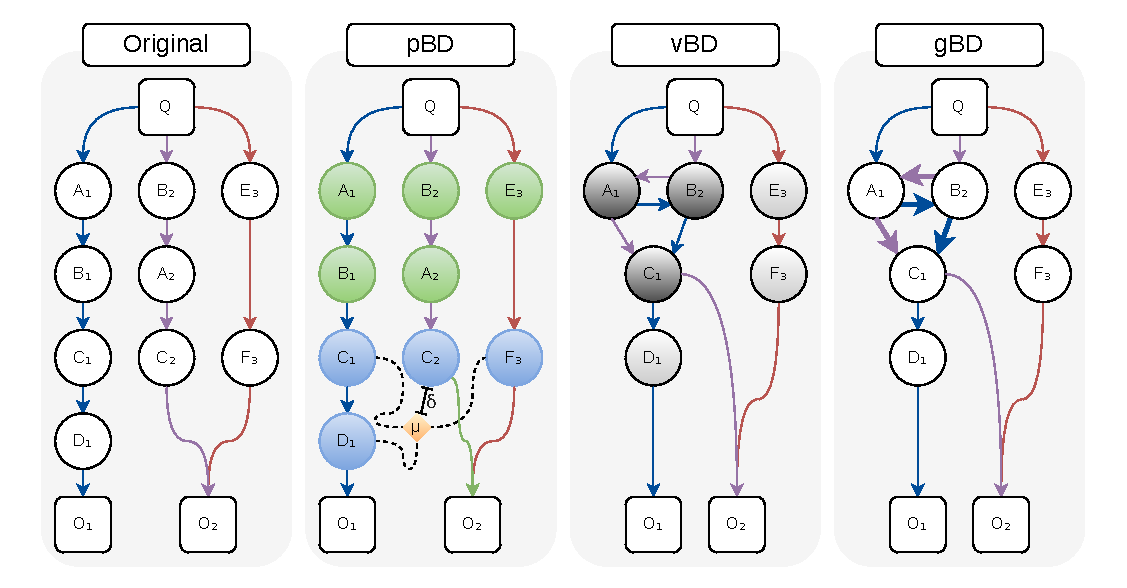
\includegraphics[width=0.95\textwidth]{resources/methods_overview}
  \caption{Overview of the three band-depth estimators on a toy ensemble of CoT
  chains (\textbf{Original}: raw sampled chains from input $Q$ to answers
  $O_1, O_2$). \textbf{pBD} DTW-aligns the chains by step position and scores each
  step by its centroid distance $\delta = 1 - \cos(e(s_k), \mu_k)$ to the aligned
  centroid $\mu_k$; a chain's depth is its mean closeness to those centroids.
  \textbf{vBD} builds the reasoning graph (vertices $A$--$F$) and shades each node
  by its vertex band depth---how often it falls inside the geodesic hull of random
  vertex pairs (dark = central, light = peripheral)---scoring a chain by the mean
  depth of the nodes it visits. \textbf{gBD} returns to the path level, scoring a
  chain by how centrally its whole trajectory runs through the graph relative to
  sampled random walks (colored arrows): a path threading the dense core scores
  deeper than one skirting the fringe.}
  \label{fig:methods}
\end{figure*}

We now develop a family of black-box confidence scorers that act on the ensemble
of reasoning chains $\{P_i^{(m)}\}_{m=1}^{M}$ defined in
Section~\ref{sec:prelim}. The common principle is \emph{centrality}: a reasoning
chain that lies deep within the ensemble---surrounded and ``enclosed'' by the
others---reflects a stable, well-supported line of reasoning, whereas an
outlying chain signals instability. We make this precise through band depth and
present three estimators of increasing structural sophistication: pBD
(Section~\ref{sec:method:pbd}), vBD (Section~\ref{sec:method:vbd}), and gBD
(Section~\ref{sec:method:gbd}). For brevity we drop the prompt index $i$ and
write the ensemble as $\{P^{(1)}, \ldots, P^{(M)}\}$, with $P^{(m)} = (s_1^{(m)},
\ldots, s_{n_m}^{(m)})$ and step embeddings $e(s_j^{(m)}) \in \mathbb{R}^d$.

\paragraph{Band depth.}
Band depth is a notion from functional data analysis that ranks a sample of
curves from most central to most outlying~\citep{lopezpintado2009banddepth}.
Given a set of curves, any pair (or larger subset) delimits a \emph{band}, and
the depth of a curve is the fraction of bands that fully contain it; the curve of
maximal depth is the functional median, and low-depth curves are outliers. The
concept has been extended to ensembles of contours~\citep{santer2023contourbanddepth}
and of paths on a graph~\citep{raj2017pathboxplots}. We adapt these ideas to
reasoning chains: each chain plays the role of a curve, and its depth within the
ensemble serves as a confidence signal---high ensemble depth indicates agreement
and reliability, low depth indicates dispersion and uncertainty.



\subsection{pBD: Path Band Depth}
\label{sec:method:pbd}

pBD treats each reasoning chain as an \emph{ordered} sequence of step embeddings
and measures how close a chain runs to the ensemble's central tendency at each
position. Because chains have different lengths and may reason at different
paces, we align them with Dynamic Time Warping (DTW) before comparison.

For a chain $P^{(m)}$ and every other chain $P^{(r)}$ ($r \neq m$), let
$\sigma_r$ be the DTW alignment mapping each step index $k$ of $P^{(m)}$ to its
corresponding index in $P^{(r)}$. At each step index $k$ we form the
\emph{aligned centroid} of the other chains' matched steps,
\begin{equation}
  \mu_k^{(m)} = \frac{1}{M-1} \sum_{r \neq m} e\big(s_{\sigma_r(k)}^{(r)}\big),
\end{equation}
and measure the \emph{centroid distance} $\delta_k^{(m)}$ of $s_k^{(m)}$ to that
centroid (the quantity drawn in the pBD panel of Figure~\ref{fig:methods}),
\begin{equation}
  \delta_k^{(m)} = 1 - \cos\!\big( e(s_k^{(m)}),\, \mu_k^{(m)} \big) \in [0, 1],
\end{equation}
so that a small $\delta_k^{(m)}$ means $s_k^{(m)}$ sits close to the ensemble's
consensus at position $k$. The path depth of $P^{(m)}$ is its mean closeness to
the centroids,
\begin{equation}
  s^{(m)} = \frac{1}{n_m} \sum_{k=1}^{n_m} \big( 1 - \delta_k^{(m)} \big),
\end{equation}
and the ensemble-mean depth $\bar{s} = \frac{1}{M} \sum_{m=1}^{M} s^{(m)}$ is
then combined with answer agreement to form the final confidence through the
shared blend of Eq.~\eqref{eq:blend}.

Despite capturing uncertainty in the CoT chain, pBD has its own weakness. In
Table~\ref{tab:ensemble-example}, two chains were produced for a single HotpotQA
question and both reach the correct answer ``We Are the Ocean'' through the same
four-step logic---look up each band's member count, compare the two numbers, and
conclude. The chains are identical in length and wording and differ \emph{only}
in the \emph{order} of the two member-count lookups: Chain~A states ``We Are the
Ocean'' first, Chain~B states ``The Dream Academy'' first. Conceptually the two
chains are the same, but pBD compares step embeddings position by position, so it
aligns ``We Are the Ocean has 5 members'' (Chain~A, step~1) against ``The Dream
Academy has 3 members'' (Chain~B, step~1) and registers large spurious diversity,
deflating the depth exactly where confidence should be highest. pBD is therefore
\emph{order-sensitive}, even though agreement among reasoning chains is inherently
order-invariant. Computationally, aligning every pair of chains with DTW costs
$O(n^2 d)$ per pair and $O(M^2 n^2 d)$ for the full ensemble. Both problems stem
from insisting on a position-wise, sequential view of the chains.

\begin{table}[t]
  \centering
  \footnotesize
  \setlength{\tabcolsep}{6pt}
  \begin{tabular}{c|ll}
    \toprule
    Step & \textbf{Chain A} & \textbf{Chain B} \\
    \midrule
    1 & WATO has 5 members & TDA has 3 members \\
    2 & TDA has 3 members  & WATO has 5 members \\
    3 & $5 > 3$            & $5 > 3$ \\
    4 & WATO is larger     & WATO is larger \\
    \bottomrule
  \end{tabular}
  \caption{Two Chain-of-Thought chains for the HotpotQA question
  \emph{``Which band has more members, We Are the Ocean or The Dream Academy?''}
  (WATO = We Are the Ocean, TDA = The Dream Academy). Both chains have the same
  length and the same reasoning; they differ \emph{only} in the order of the two
  member-count lookups (steps 1--2). pBD's position-wise comparison nonetheless
  aligns ``WATO has 5 members'' (Chain~A, step~1) against ``TDA has 3 members''
  (Chain~B, step~1) and counts the two chains as diverse, motivating the
  order-invariant graph of Section~\ref{sec:method:graph}.}
  \label{tab:ensemble-example}
\end{table}

\subsection{Reasoning Graph Construction}
\label{sec:method:graph}

To mitigate both the order-sensitivity and the alignment cost of pBD, we abandon
position-wise comparison and instead collapse the ensemble into a single
\emph{reasoning graph} $G = (V, E)$, which is used later in vBD and gBD. By merging
semantically equivalent steps into shared nodes regardless of where they appear
in a chain, the graph maps the reordered lookups of
Table~\ref{tab:ensemble-example} onto one shared structure: equivalent reasoning
is no longer counted as diversity and no pairwise alignment is needed. Starting from the embedded steps of all $M$
chains:
\begin{itemize}
  \item \textbf{Nodes.} Steps whose pairwise cosine similarity exceeds a high
        threshold $\theta_c$ are merged into a single node, so that each
        $v \in V$ represents a semantic cluster of equivalent reasoning states.
  \item \textbf{Sequential edges.} Consecutive steps within the same chain are
        joined by a directed edge, preserving local reasoning flow.
  \item \textbf{Semantic edges.} Steps from different chains whose cosine
        similarity exceeds a lower threshold $\theta_e < \theta_c$ are joined by
        an undirected edge, linking related reasoning across chains.
\end{itemize}
Each reasoning chain $P^{(m)}$ thereby becomes a walk over $V$, and the geometry
of the ensemble is encoded in the topology of $G$.

\subsection{vBD: Vertex Band Depth}
\label{sec:method:vbd}

vBD measures the \emph{centrality of each individual vertex} in the reasoning
graph (the vBD panel of Figure~\ref{fig:methods}), and then scores a chain by how
central the nodes it visits are. A vertex is central if it lies ``between'' many other reasoning
states---a node that the bulk of the graph encloses---and peripheral if it sits
at the fringe. Because
only the \emph{set} of visited nodes enters the score, vBD is fully
order-invariant. Concretely, we sample vertex pairs uniformly from the vertex set $V$. For a
vertex $v$, its vertex band depth is the probability that $v$ lies inside the
geodesic convex hull $H[\cdot]$ of two vertices
$\mathcal{V}_2 = \{v_a, v_b\}$ drawn at random from $V$,
\begin{equation}
  v\text{BD}(v) = \mathbb{E}_{\mathcal{V}_2 \sim V}\!\left[ \mathbf{1}\big(v \in H[\mathcal{V}_2]\big) \right],
\end{equation}
estimated by Monte Carlo sampling of $S$ such pairs from $V$. The depth of a
chain is the mean vertex depth over the nodes it visits,
\begin{equation}
  c\text{BD}\big(P^{(m)}\big) = \frac{1}{|P^{(m)}|} \sum_{v \in P^{(m)}} v\text{BD}(v),
\end{equation}
and the ensemble-mean depth $\bar{s} = \frac{1}{M} \sum_{m=1}^{M} c\text{BD}(P^{(m)})$
again enters the shared confidence blend of Eq.~\eqref{eq:blend}.

Beyond graph construction, vBD requires only $S$ sampled vertex pairs from $V$,
each needing a geodesic-hull membership test, and is far cheaper than pBD's
pairwise DTW. Its limitation is that it treats each vertex \emph{independently}:
by averaging per-vertex depths it ignores how those vertices are linked into a
path---the transitions a chain takes and the order in which it visits states.
Two chains that occupy the same set of central nodes but connect them through
very different reasoning receive the same vBD score, even if one follows a
coherent route through the graph and the other jumps erratically between
unrelated states. vBD thus captures \emph{which} reasoning states a chain
occupies but not \emph{how} it moves among them.

\subsection{gBD: Graph Band Depth}
\label{sec:method:gbd}

gBD, our main method, returns depth to the \emph{path} level while remaining
order-invariant, recovering exactly the information vBD discards: the relations
between steps---which reasoning states follow which, and how a chain threads them
together. Whereas vBD asks only whether a chain's individual nodes are central,
gBD asks whether the chain's whole \emph{trajectory} through the graph is central.
A chain that visits central nodes but connects them through incoherent jumps is
no longer scored as though it reasoned coherently, because its transitions, not
just its nodes, are evaluated.

gBD also differs fundamentally from pBD in its \emph{reference distribution}. pBD
can compare only the $M$ chains the model actually sampled, aligned pairwise; it
never considers any reasoning beyond those $M$. Our graph, by contrast, clusters
semantically equivalent steps into shared nodes and links steps across chains
with edges, so it encodes reasoning transitions that no \emph{single} sampled
chain exhibits. A random walk on $G$ can traverse these edges to synthesize
entirely new chains. As the gBD panel of Figure~\ref{fig:methods} illustrates,
gBD scores a chain by how centrally its whole \emph{trajectory} runs through the
graph: a path that threads the dense core ($Q \to A \to B \to C \to D \to O_1$)
attains higher depth than a peripheral path that skirts the fringe
($Q \to E \to F \to O_1$), even though both are valid input-to-output routes. gBD draws random walks as its
reference paths, so it measures a chain's depth against the full reasoning space
the graph defines rather than against only the $M$ observed chains. This yields a
markedly richer depth estimate that remains robust when the ensemble is small,
because the graph interpolates reasoning paths the model did not happen to sample.

For each real chain $P^{(m)}$ we draw $T$ pairs of random walks
$(W_a^{(t)}, W_b^{(t)})$ on $G$ and measure the fraction of $P^{(m)}$'s vertices
that fall inside the geodesic convex hull of each pair (soft containment),
averaged over the $T$ draws,
\begin{equation}
  \text{gBD}\big(P^{(m)}\big) = \frac{1}{T} \sum_{t=1}^{T}
  \frac{\big|\{\, v \in P^{(m)} : v \in \text{hull}(W_a^{(t)}, W_b^{(t)}) \,\}\big|}{|P^{(m)}|}.
\end{equation}
The final confidence blends the mean depth $\bar{s}$ with the answer-level
majority fraction $\rho$ (the share of chains agreeing with the modal answer),
\begin{equation}
\label{eq:blend}
  \hat{s} = \alpha \, \bar{s} + (1 - \alpha)\, \rho.
\end{equation}
For gBD $\bar{s} = \overline{\text{gBD}} = \frac{1}{M}\sum_m \text{gBD}(P^{(m)})$,
and the same form of blend is applied to all three estimators, substituting the
corresponding depth score $\bar{s}$ of pBD or vBD. The weight $\alpha$ trades
reasoning-structure depth against answer agreement: in our main results we use
$\alpha = 0.9$ for pBD and vBD and $\alpha = 0.3$ for gBD, whereas the ablation
study (Section~\ref{sec:exp:ablation}) holds $\alpha = 0.5$ fixed across methods
to isolate the remaining hyperparameters. We consider two variants for generating
the reference walks:
\begin{itemize}
  \item \textbf{gBD-v1 (anchored):} walks are constrained to start at the graph's
        input node and end at its output node, following the global
        question-to-answer direction.
  \item \textbf{gBD-v2 (free):} walks may start and end anywhere in $G$, freely
        exploring its topology; this is our strongest estimator.
\end{itemize}

gBD draws $T$ walk pairs per chain and performs hull-membership tests, comparable
in cost to vBD and far below pBD. By sampling reference paths absent from the
ensemble, gBD obtains a richer depth estimate that is robust to small ensembles,
captures path-level structure, and is order-invariant---combining the strengths
of pBD and vBD.

% -----------------------------------------------------------------------
\section{Related Works}
\label{sec:related}

\subsection{Black-box Uncertainty Quantification for LLMs}
The dominant black-box paradigm estimates uncertainty from the consistency of
multiple sampled responses. Self-consistency takes the agreement of the majority
answer as a confidence signal~\citep{wang2023selfconsistency}, while semantic
uncertainty and semantic entropy cluster responses by meaning and measure the
entropy of the resulting distribution~\citep{kuhn2023semantic, farquhar2024detecting}.
A related family scores the original response against samples through pairwise
measures---exact-match and non-contradiction rates, BERTScore or embedding-cosine
similarity, and normalized semantic negentropy~\citep{lin2023generating}---while
SelfCheckGPT applies the same intuition to hallucination detection without
external resources~\citep{manakul2023selfcheckgpt}. Other work calibrates answers
from arbitrary models via sampling agreement~\citep{chen2024quantifying} or uses
sampling to decide when to abstain on ambiguous
questions~\citep{stelmakh2022selectively}. A complementary line elicits confidence
from the model in natural language: \citet{xiong2024llms} study prompting,
sampling, and aggregation strategies---vanilla, chain-of-thought, top-$k$,
multi-step, and self-probing prompts---and find LLMs markedly overconfident, an
effect prompting only partially mitigates, while other work instruction-tunes
models to express calibrated confidence on self-generated
labels~\citep{liu2024uait}.

A more recent line moves beyond the final answer toward the reasoning itself.
Closest to us, CoT-UQ extracts keywords from each reasoning step, scores their
importance, and reweights token probabilities accordingly~\citep{zhang2025cotuq};
it nonetheless requires access to token logits and operates on a single response
rather than an ensemble. Graph-based metrics summarize relationships among claims
extracted from long-form generations~\citep{jiang2024graphuncertainty}, targeting
factuality rather than the geometry of reasoning, and further approaches estimate
uncertainty through multi-agent interaction across query
variations~\citep{feng2025multiagent}, iterative
prompting~\citep{abbasiyadkori2024believe}, cross-model
disagreement~\citep{hamidieh2026crossmodel}, or interrogative probing of long-form
outputs~\citep{fan2026iuq}. All of these summarize the distribution of final
answers or claims, or rely on the model's own introspection; none characterizes
the \emph{structural centrality} of an ensemble of reasoning chains, which is the
signal our methods exploit. Our approach is fully black-box (text only, requiring
no token logits), operates on an ensemble, extracts its signal geometrically
rather than by introspection, and adds no LLM calls beyond the initial sampling.

\subsection{Band Depth and Contour Ensembles}
Our geometric tools originate in functional data analysis, where band depth
provides a center-outward ordering of curves and identifies a functional
median~\citep{lopezpintado2009banddepth}. A substantial body of visualization
research has since extended depth to spatial ensembles. Contour band depth
generalizes the notion to ensembles of contours and underlies box-and-whisker
style summaries of two-dimensional uncertainty~\citep{santer2023contourbanddepth};
inclusion depth offers an efficient alternative based on inside/outside
relationships between contours~\citep{chavesdeplaza2024inclusiondepth}, and
further work handles multi-modal ensembles by disentangling their modes of
variation~\citep{chavesdeplaza2024multimodal}. Most relevant to us, band depth has
been generalized to ensembles of \emph{paths on a graph}, yielding a
center-outward ordering of paths and a corresponding path
boxplot~\citep{raj2017pathboxplots}. We build directly on this path-on-graph
formulation, but repurpose it: rather than visualizing ensemble uncertainty, we
treat the sampled reasoning chains of an LLM as the path ensemble and use their
depth as a black-box confidence score. To our knowledge, this is the first
application of band depth to LLM reasoning for uncertainty quantification.

% -----------------------------------------------------------------------
\section{Experiments}
\label{sec:exp}

\subsection{Experimental Setup}
\label{sec:exp:setup}

\textbf{Datasets.} We evaluate on five reasoning benchmarks spanning two regimes.
For mathematical reasoning we use GSM8K~\citep{cobbe2021gsm8k},
SVAMP~\citep{patel2021svamp}, and ASDiv~\citep{miao2020asdiv}, where correctness
is determined by exact match against the gold numerical answer. For multi-hop
question answering we use HotpotQA~\citep{yang2018hotpotqa} and
2WikiMultihopQA~\citep{ho2020wikimultihop}; following common practice for
open-ended answers, correctness is judged by an LLM grader. For 2WikiMultihopQA
we restrict to the \emph{inference} question type.

\textbf{Models.} We use two open-weight backbones of different family and scale,
Llama-3.1-8B~\citep{grattafiori2024llama3} and
Llama-2-13B~\citep{touvron2023llama2}, applying the same step-wise CoT prompt to
both. For every question we sample an ensemble of $M = 5$ reasoning chains under
temperature decoding, which forms the common input to all ensemble-based scorers.

\textbf{Baselines.} We compare against two families of black-box scorers. The
first is \emph{CoT-UQ}~\citep{zhang2025cotuq}, a verbalized self-probing
method~\citep{xiong2024llms} in which the model is asked to state the probability
that its own answer is correct. It has five prompting variants---the vanilla
probe and four reasoning-augmented forms that condition on extracted keywords
(\textsc{KeyWords}, \textsc{AllKeyWords}) or reasoning steps (\textsc{KeyStep},
\textsc{AllStep})---of which we report the best-performing variant per dataset as
a single \textsc{CoT-UQ} entry. The second family is
\emph{sampling-based consistency}, which scores the ensemble by answer agreement:
Non-Contradiction probability and Entailment probability, both computed with an
NLI model, and Semantic Entropy~\citep{kuhn2023semantic, farquhar2024detecting}.

\textbf{Our methods and encoder.} We report all four band-depth estimators---pBD,
vBD, gBD-v1, and gBD-v2---computed on the same ensemble. Reasoning steps are
embedded with the all-MiniLM-L6-v2 sentence encoder~\citep{reimers2019sentencebert};
the graph-depth blending weight is fixed to $\alpha = 0.10$, and the similarity
thresholds $\theta_c, \theta_e$ and walk count $T$ are held constant across all
datasets. None of our methods issue any LLM call beyond the initial ensemble.

\textbf{Metric.} Following standard practice~\citep{kuhn2023semantic, xiong2024llms},
we report AUROC ($\times 100$) between each scorer's confidence and binary answer
correctness, where 50 denotes random ranking and higher is better.

\subsection{Main Results}
\label{sec:exp:main}

Table~\ref{tab:main-results} reports AUROC for all methods. The band-depth family
dominates across both models and all five datasets, and gBD-v2 is the strongest
scorer in nearly every column. On Llama-3.1-8B, gBD-v2 reaches 77.19 on HotpotQA,
76.12 on ASDiv, and 74.81 on SVAMP, improving over the best sampling baseline by
roughly 13.4, 3.7, and 5.6 points respectively, and over CoT-UQ by more than 20
points on HotpotQA. On Llama-2-13B, where the gains are
even larger, gBD-v2 attains 73.13 on GSM8K and 70.74 on SVAMP, exceeding CoT-UQ
by roughly 20 points. The only benchmark not won by a gBD
variant is 2WikiMultihopQA, where vBD leads on both models (69.22 on Llama-3.1-8B,
73.60 on Llama-2-13B); we return to this case below.

\begin{table*}[t]
  \centering
  \footnotesize
  \setlength{\tabcolsep}{6pt}
  \begin{tabular}{c l cc ccc}
    \toprule
    \multirow{2}{*}{\textbf{Model}} & \multirow{2}{*}{\textbf{Method}}
      & \multicolumn{2}{c}{\textbf{Multi-hop QA}}
      & \multicolumn{3}{c}{\textbf{Mathematical Reasoning}} \\
    \cmidrule(lr){3-4}\cmidrule(lr){5-7}
      & & HotpotQA & 2WikiMHQA & GSM8K & SVAMP & ASDiv \\
    \midrule
    \multirow{8}{*}{\textbf{Llama-3.1-8B}}
      & CoT-UQ                  & 54.92 & 56.67 & 54.58 & 54.35 & 51.77 \\
    \cmidrule(lr){2-7}
      & Non-Contradiction       & 58.62 & 58.54 & 57.49 & 64.34 & 66.40 \\
      & Entailment Prob.        & 63.78 & 58.32 & 63.72 & 69.22 & 72.41 \\
      & Semantic Entropy        & 62.33 & 52.98 & 60.80 & 62.82 & 67.05 \\
    \cmidrule(lr){2-7}
      & pBD                     & 76.29 & 62.31 & 65.99 & 69.49 & 72.61 \\
      & vBD                     & 76.16 & \textbf{69.22} & 64.90 & 67.14 & 69.77 \\
      & gBD-v1                  & 77.05 & 67.73 & 68.08 & 74.76 & 76.02 \\
      & gBD-v2                  & \textbf{77.19} & 68.39 & \textbf{68.69} & \textbf{74.81} & \textbf{76.12} \\
    \midrule
    \multirow{8}{*}{\textbf{Llama-2-13B}}
      & CoT-UQ                  & 67.43 & 57.06 & 53.02 & 51.25 & 56.23 \\
    \cmidrule(lr){2-7}
      & Non-Contradiction       & 63.99 & 67.74 & --    & --    & 65.87 \\
      & Entailment Prob.        & 68.03 & 64.28 & --    & --    & 72.70 \\
      & Semantic Entropy        & 63.51 & 59.27 & --    & --    & 66.00 \\
    \cmidrule(lr){2-7}
      & pBD                     & 74.83 & 62.64 & 72.29 & 67.60 & 74.41 \\
      & vBD                     & 73.84 & \textbf{73.60} & 69.47 & 66.22 & 71.40 \\
      & gBD-v1                  & 77.76 & 73.24 & 72.86 & 70.53 & 76.22 \\
      & gBD-v2                  & \textbf{78.04} & 73.12 & \textbf{73.13} & \textbf{70.74} & \textbf{76.51} \\
    \bottomrule
  \end{tabular}
  \caption{AUROC ($\times 100$, $\uparrow$) for black-box UQ on five reasoning
  benchmarks. Best result per column (within a model) is in \textbf{bold}.
  Entries marked ``--'' are the Llama-2-13B sampling baselines
  (Non-Contradiction, Entailment, Semantic Entropy) on GSM8K and SVAMP, which
  remain pending [TODO: run experiment].}
  \label{tab:main-results}
\end{table*}

\subsection{Analysis}
\label{sec:exp:analysis}

\textbf{gBD is the strongest band-depth variant overall.} Comparing our three
estimators, the graph-level gBD attains the best AUROC in 9 of the 10
model--dataset columns, and the free-walk gBD-v2 edges out the anchored gBD-v1 in
nearly every column (the sole exception being 2WikiMultihopQA on Llama-2-13B,
where the two are within 0.1 point). gBD's advantage is most pronounced on
mathematical reasoning---on SVAMP it improves over pBD and vBD by 5.3 and 7.7
points respectively (Llama-3.1-8B)---confirming the central design choice of gBD:
scoring a chain against random reference walks over the full graph topology,
rather than against only the sampled chains, yields a richer and more
discriminative depth estimate.

\textbf{vBD is better suited to short-chain multi-hop reasoning.} The one regime
where gBD does not lead is 2WikiMultihopQA, where the vertex-level vBD is the
strongest band-depth variant on both models (69.22 on Llama-3.1-8B, 73.60 on
Llama-2-13B), outscoring both gBD variants. We attribute this to the subset's
short inference chains, which yield sparse reasoning graphs on which per-vertex
centrality is more stable than path-level random walks; once chains are long
enough to form a richly connected graph---the mathematical and HotpotQA
settings---gBD's path-level view dominates.

\textbf{Order-sensitivity holds pBD back.} The path-aligned pBD is competitive
where reasoning is largely linear (e.g.\ HotpotQA, 76.29 on Llama-3.1-8B) but
falls furthest behind on 2WikiMultihopQA (62.31 and 62.64), whose multi-hop
chains frequently reorder commutative lookups. Because pBD compares step
embeddings position by position, it penalizes these reorderings as spurious
diversity---the failure mode of Table~\ref{tab:ensemble-example}---which the
order-invariant vBD and gBD avoid (see the controlled comparison in
Section~\ref{sec:exp:ablation}).

\subsection{Ablation Study}
\label{sec:exp:ablation}

The progression pBD $\rightarrow$ vBD $\rightarrow$ gBD in
Table~\ref{tab:main-results} doubles as an ablation over the two core design
decisions. \emph{Order-invariance:} moving from the order-sensitive pBD to the
graph-based methods removes the artificial penalty on commutative reasoning;
this helps most on 2WikiMultihopQA, where vBD improves over pBD by 6.9 points
(62.31 $\rightarrow$ 69.22). \emph{Reference distribution:} replacing
ensemble-only references with random walks over the graph (gBD) restores
path-level sensitivity that vBD discards, lifting AUROC on every mathematical
dataset---for example on SVAMP, gBD-v2 improves over vBD by 7.7 points
(67.14 $\rightarrow$ 74.81). Together these show that both ingredients
contribute, and that gBD's combination of order-invariance with a graph-derived
reference is what makes it the strongest estimator overall. The anchored/free
contrast (gBD-v1 vs.\ gBD-v2) further isolates the value of unconstrained walks,
which consistently provide a small additional gain.

We further isolate the hyperparameters specific to the band-depth construction:
the band \emph{subset size}, the gBD \emph{random-walk length}, the two graph
similarity \emph{thresholds}, and the number of Monte-Carlo \emph{trials}. To keep
the study tractable, all ablations below are run on a single representative
dataset---SVAMP, the smallest benchmark---with Llama-3.1-8B, and fix the
confidence blend weight at $\alpha = 0.5$. Each sweep recomputes band depth on the
same fixed sampled ensembles as the main results and writes its AUROCs to a
separate \texttt{output/ablation/} location, leaving \texttt{output/metric/}
untouched. The results (Table~\ref{tab:ablation})
show the method to be highly stable: AUROC varies within roughly one point across
every sweep. The clustering threshold $\theta_c$ is the only setting with a
pronounced effect---low values over-merge distinct reasoning steps and degrade
vBD by over two points (74.82 at $\theta_c{=}0.92$ down to 72.37 at $0.85$)---
confirming that the chosen defaults ($J{=}2$, $\theta_c{=}0.92$, $\theta_e{=}0.70$,
$T{=}200$) are well calibrated.

\subsubsection{Band Subset Size}
\label{sec:exp:ablation:subset}

Band depth is defined relative to ``bands'' delimited by random subsets of the
ensemble. Our default estimators use the smallest such subset: vBD draws pairs of
vertices and tests whether a target vertex lies in their geodesic hull, while gBD
draws pairs of reference walks. The subset size $J$ controls how large each band
is---larger $J$ produces wider hulls that enclose more of the graph, trading
sensitivity for stability---so it is the natural first hyperparameter to ablate.
Table~\ref{tab:ablation} (subset-size block) sweeps $J \in \{2,3,4,5\}$ for both
vBD and gBD-v2, holding all else fixed, to determine whether the minimal pairwise
band is in fact the best choice.

% Results written to output/ablation/{subset_size,walk_length,sim_threshold,cross_threshold,trials}.json
\begin{table}[t]
  \centering
  \footnotesize
  \begin{tabular}{l l cc}
    \toprule
    Hyperparameter & Setting & \textbf{vBD} & \textbf{gBD-v2} \\
    \midrule
    \multirow{4}{*}{Subset size $J$}
       & 2 (default)     & \textbf{74.74} & 74.52 \\
       & 3               & 74.27 & 74.68 \\
       & 4               & 74.16 & 74.78 \\
       & 5               & 74.06 & \textbf{74.80} \\
    \midrule
    \multirow{5}{*}{Walk length $L$}
       & 3               & --    & 74.71 \\
       & 5               & --    & 74.85 \\
       & 7               & --    & \textbf{74.90} \\
       & 10              & --    & 74.88 \\
       & adaptive (default) & -- & 74.52 \\
    \midrule
    \multirow{5}{*}{Cluster thr.\ $\theta_c$}
       & 0.85            & 72.37 & 74.26 \\
       & 0.88            & 73.63 & \textbf{74.82} \\
       & 0.90            & 74.01 & 74.41 \\
       & 0.92 (default)  & \textbf{74.82} & 74.47 \\
       & 0.95            & 74.81 & 74.74 \\
    \midrule
    \multirow{5}{*}{Edge thr.\ $\theta_e$}
       & 0.60            & --    & \textbf{74.71} \\
       & 0.65            & --    & 74.68 \\
       & 0.70 (default)  & --    & 74.52 \\
       & 0.75            & --    & 74.21 \\
       & 0.80            & --    & 74.27 \\
    \midrule
    \multirow{4}{*}{MC trials $T$}
       & 50              & 74.60 & \textbf{74.61} \\
       & 100             & \textbf{74.76} & 74.52 \\
       & 200 (default)   & 74.73 & 74.61 \\
       & 400             & 74.72 & 74.54 \\
    \bottomrule
  \end{tabular}
  \caption{Band-depth ablations on SVAMP, Llama-3.1-8B, AUROC ($\times 100$).
  Each block sweeps one hyperparameter with all others held at their default
  (marked ``default''). ``--'' marks settings that do not apply to vBD: the
  walk length $L$ and semantic-edge threshold $\theta_e$ are gBD-only. Default
  configuration: $J{=}2$, $L$ adaptive, $\theta_c{=}0.92$, $\theta_e{=}0.70$,
  $T{=}200$.}
  \label{tab:ablation}
\end{table}

\subsubsection{Random-Walk Length in gBD}
\label{sec:exp:ablation:walklen}

gBD's reference paths are random walks over the reasoning graph, and their length
$L$ governs how much of the graph each reference path spans: walks that are too
short cannot enclose a full reasoning chain, while walks that are too long wander
across unrelated regions and dilute the depth signal. There should therefore be
an intermediate length matched to the typical chain length that is most
discriminative. Table~\ref{tab:ablation} (walk-length block) sweeps $L$ over a
range of fixed values together with the current adaptive default (length scaled
to the graph), for gBD-v2.

\subsubsection{Graph Construction Thresholds}
\label{sec:exp:ablation:thresh}

The reasoning graph depends on two cosine-similarity thresholds: the clustering
threshold $\theta_c$, above which two steps merge into a single node, and the
semantic-edge threshold $\theta_e$, above which steps from different chains are
joined by a soft edge. $\theta_c$ governs how aggressively the graph collapses
equivalent reasoning---set too low it over-merges distinct states, too high it
fragments the graph---while $\theta_e$ controls how densely the chains are
cross-connected. Table~\ref{tab:ablation} sweeps $\theta_c$ for both vBD and
gBD-v2 (cluster-threshold block) and $\theta_e$ for gBD-v2 (edge-threshold block;
vBD uses no soft edges).

\subsubsection{Number of Monte-Carlo Trials}
\label{sec:exp:ablation:trials}

Both estimators approximate band depth by sampling---vBD over random vertex
subsets, gBD over pairs of random walks---using $T$ trials per estimate. Larger
$T$ reduces estimator variance at a cost linear in $T$.
Table~\ref{tab:ablation} (MC-trials block) sweeps $T \in \{50, 100, 200, 400\}$
to verify that the estimates are converged at the default $T = 200$.

Finally, two items remain and are likewise flagged as [TODO: run experiment]:
sensitivity to the ensemble size $M \in \{5, 10, 20, 50\}$ (on SVAMP with
Llama-3.1-8B), to quantify how gracefully each method degrades as fewer chains
are sampled; and the Llama-2-13B sampling baselines on GSM8K and SVAMP (the
remaining ``--'' entries in Table~\ref{tab:main-results}).

% -----------------------------------------------------------------------
% References and End of Paper
\bibliography{references}

\end{document}
